\subsection{Within Database Performance Evaluation}

\subsubsection{Contactless Finger Knuckle Image Database (Version 3.0)}

The finger knuckle database \cite{fingerknuckledbv3.0} can offer contactless finger knuckle of 221 subjects, but only 104 subjects have second session samples. For each session, each subject can offer 6 samples. It is worth mentioning that the finger knuckle sample provided by this database is more challenging and closer to real world scenarios, because the finger knuckle will bend from 0 to 90 degree result in crease deformation.

\textbf{One-Session Protocol}

As for the one-session protocol, I firstly fine-tuned models on the second session 104 subjects dataset, totally $104 * 6 = 624$ images as the testing set. Then use the first session 221 subjects as the testing set result in $221*6=1326$ genuine matching scores and $221*220*6=291720$ imposter matching scores. From the Figure \ref{fkv3-one-session}, we can easily find the RFNet is the best model not only on the ROC but also on the CMC. In terms of the baseline model RFNet, our loss function TRTL can improve the matching accuracy when compare to the STTL loss function. Although the finger knuckle of the database with deformation while bend from 0 to 90 degree, the EER of the RFNet-TRTL can arrive at $2.21\%$. And as top-2 ranking, the RFNet-TRTL recognition rate is about 0.97 on the CMC. As for the rest model, EfficientNetV2-S model performance is better than FKNet and DeConvRFNet. From the performance result, if we just change the convolution layer with deformable convolution, it cannot overcome finger knuckle deformation, even the performance is dropped.

\begin{figure}[ht!]
	\centering
	\begin{subfigure}[b]{0.45\linewidth}
		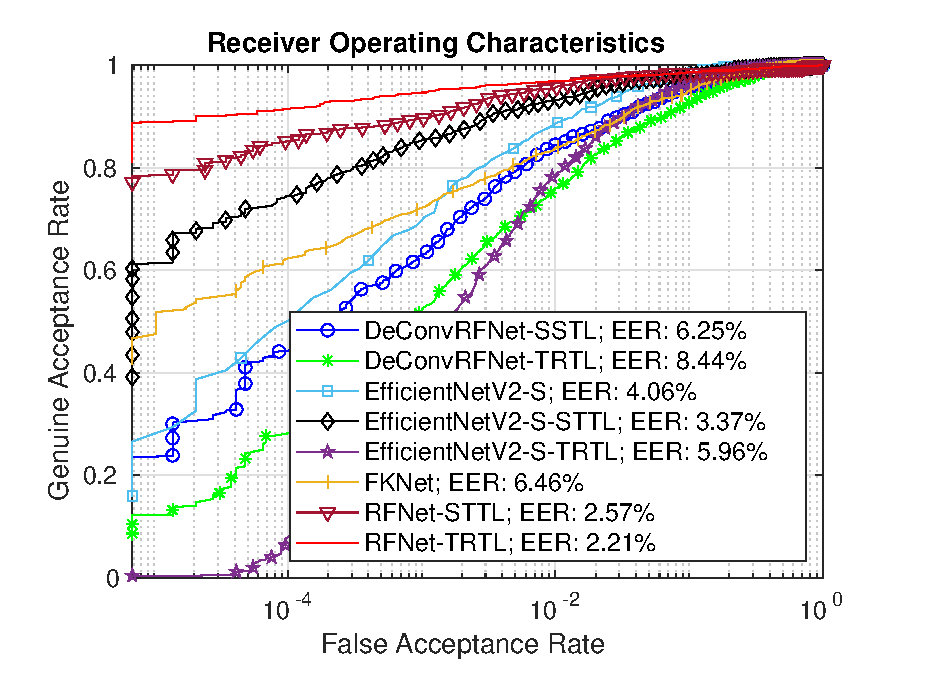
\includegraphics[width=\linewidth]{Figures/fkv3-roc_compare_new.eps}
		\caption{}
	\end{subfigure}
	\begin{subfigure}[b]{0.45\linewidth}
		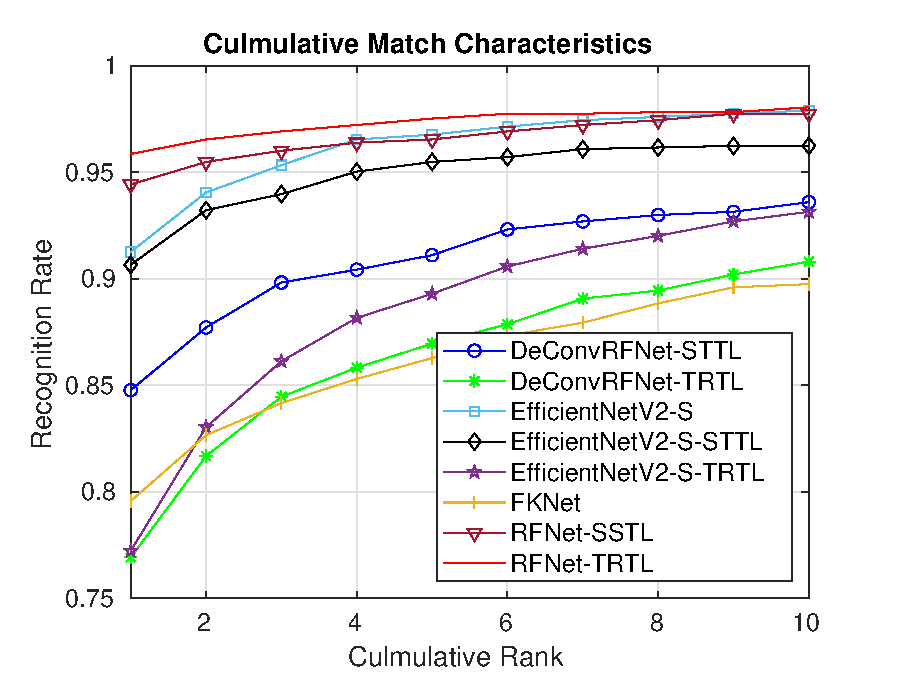
\includegraphics[width=\linewidth]{Figures/fkv3-cmc_compare_new.eps}
		\caption{}
	\end{subfigure}
	\caption{Comparative ROC (a) and corresponding CMC (b) for one-session on the contactless finger knuckle image database \cite{fingerknuckledbv3.0}.}
	\label{fkv3-one-session}
\end{figure}

\textbf{Two-Session Protocol}

We fine-tune models on the first session subjects who don't provide second session samples, and use two-session protocol to evaluate my model performance on the first session subjects who can offer two-session data. In totally, it will generate $104*6=624$ genuine scores, and $104*103*6$ imposter scores. Just like said before, the FKNet and EfficientNetV2-S are classification networks, we use output feature vector to calculate MSE as the matching score. Because the degree of deformation vary on the two-session data, the verification and identification scenarios is more complexity than one-session protocol. Due to these factors, the accuracy on the two-session protocol is much lower than the one-session protocol. However, the RFNet is still the best model, even its EER is half of the EER of other models. Meanwhile, our TRTL loss function still work better than the STTL loss function, with $16.65\%$ and $18.35\%$ respectively on the ROC. As for the CMC, when the cumulative rank value is 2, recognition rate of RFNet-TRTL can arrive at 0.7. From the ROC and CMC Figure \ref{fkv3-two-session}, we can also get that the STTL and TRTL triplet loss function are better than classification task, because the FKNet and EfficientNetV2-S have the lowest accuracy.

\begin{figure}[ht!]
    \centering
	\begin{subfigure}[b]{0.45\linewidth}
		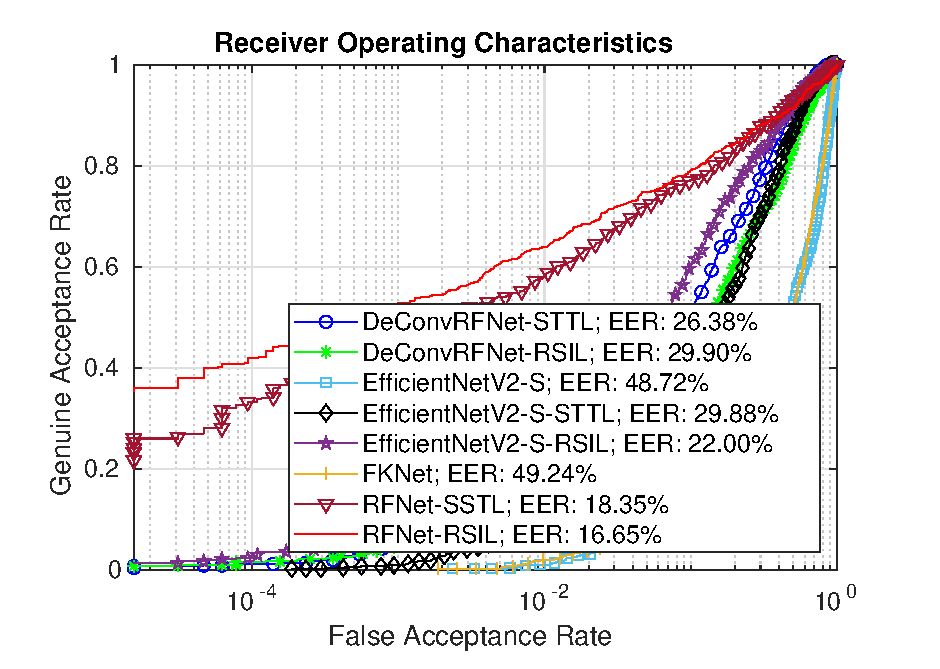
\includegraphics[width=\linewidth]{Figures/two-fkv3roc_compare_new.eps}
		\caption{}
	\end{subfigure}
	\begin{subfigure}[b]{0.45\linewidth}
		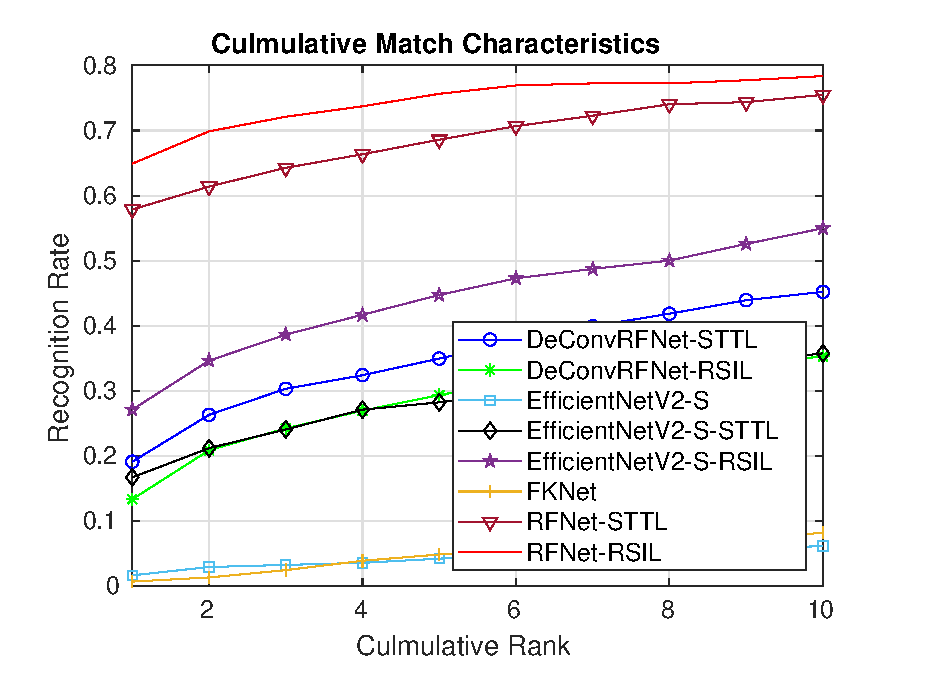
\includegraphics[width=\linewidth]{Figures/two-fkv3cmc_compare_new.eps}
		\caption{}
	\end{subfigure}
	\caption{Comparative ROC (a) and corresponding CMC (b) for two-session on the contactless finger knuckle image database \cite{fingerknuckledbv3.0}.}
	\label{fkv3-two-session}
\end{figure}


\subsubsection{Index Finger Knuckle of Contactless Hand Dorsal Image Database}

\begin{figure}[ht!]
	\centering
	\begin{subfigure}[b]{0.45\linewidth}
		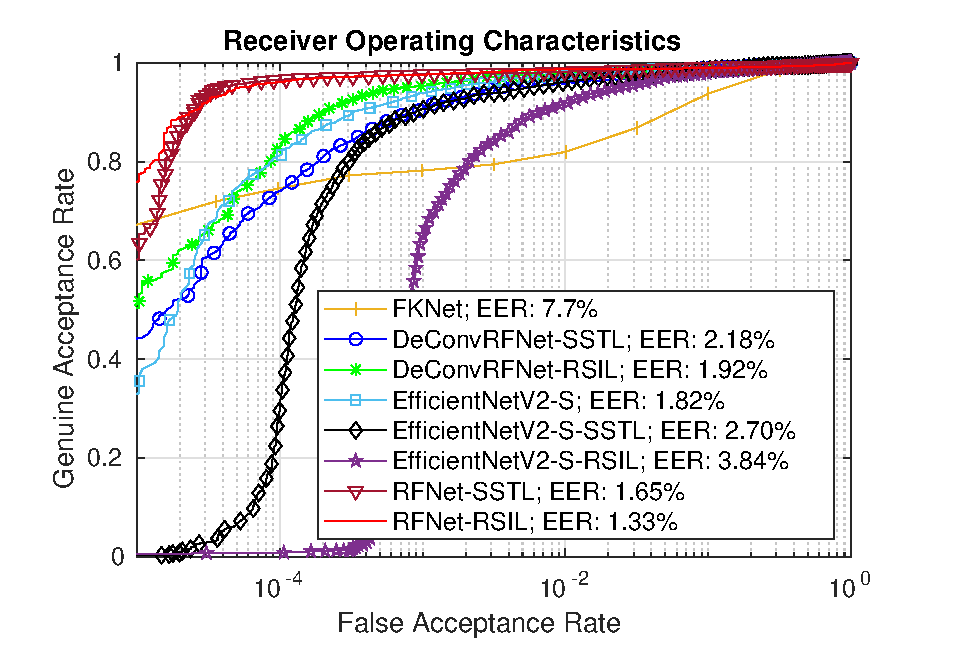
\includegraphics[width=\linewidth]{Figures/hd-roc_compare_new.eps}
		\caption{}
	\end{subfigure}
	\begin{subfigure}[b]{0.45\linewidth}
		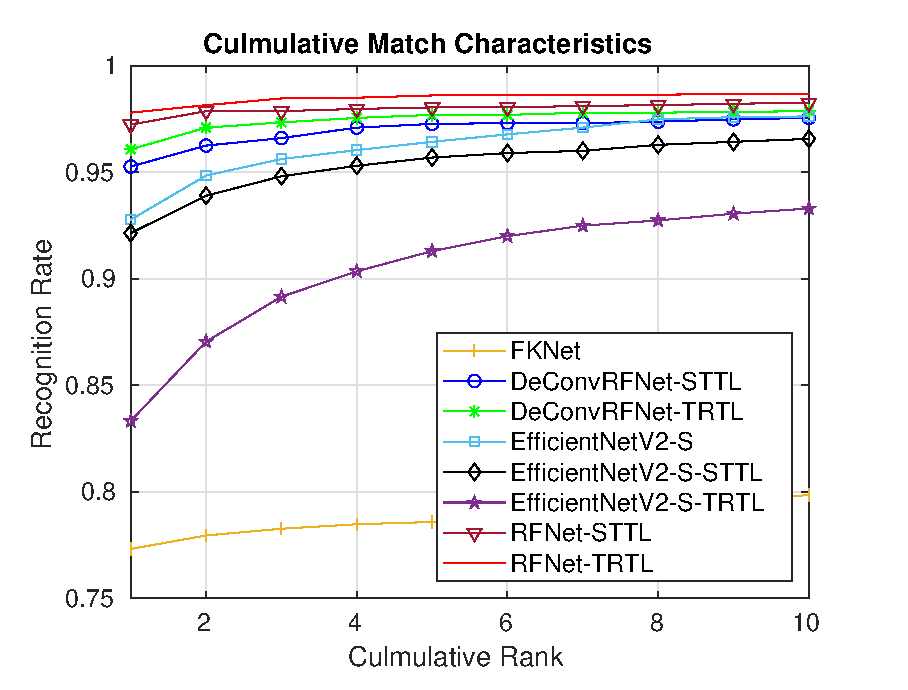
\includegraphics[width=\linewidth]{Figures/hd-cmc_compare_new.eps}
		\caption{}
	\end{subfigure}
	\caption{Comparative ROC (a) and corresponding CMC (b) for one-session on the contactless hand dorsal image database \cite{ContactlessHnadDorsaldb}.}
	\label{hd-one-session}
\end{figure}

As for the experiment, the dataset \cite{ContactlessHnadDorsaldb} totally contains 712 subjects, and each subject have 5 finger knuckle samples. And we fine-tuned our models on the first sample of each subject, and then use the rest four sample as the testing dataset. For protocol on the database, we use protocol as same as protocol of the FKNet \cite{cheng2020deep}. At the evaluation process, it has $712*4=2848$ genuine matching scores, and has $712*711*4=2024928$ imposter matching scores. The performance of RFNet-TRTL and RFNet-STTL is similar, but the RFNet-TRTL is slightly better than RFNet-STTL depend on the EER value on ROC. And on the CMC, the RFNet-TRTL still get the best accuracy. We can notice that the FKNet get the worst result when compare to other models. The EfficientNetV2-S model is still better than the FKNet, because EfficientNetV2-S is deeper than FKNet with MBConv block. MBConv block is more robust than the original residual block.


\subsubsection{2D Forefinger of 3D Finger Knuckle Database}

The HKPolyU 3D Finger Knuckle Images Database \cite{3dfingerknuckle} can offer reliable 3D finger knuckle pattern (surface normal vector, depth, or curvature) from 2D finger knuckle images, therefore we use its 2D images as our evaluation database. 190 subjects of the database have two-session finger knuckle samples, and 38 subjects offer one-session images. In this kind of situation, two-session protocol is not fit on the database, then we use one-session protocol to evaluate performance. We use the first session 190 subjects images to fine-tune models and then to test on the second session 190 subjects. It has $190*6=1140$ genuine matching scores and $190*189*6=215460$ imposter matching scores. From the ROC and CMC, we can get a conclusion that the performance of RFNet, DeConvRFNet, and EfficientNetV2-S are similar. However, the FKNet is still the worst one, which EER is $5.74\%$ and the CMC is lower than others. The unchanged thing is that the RFNet with TRTL loss still get the best performance with $1.60\%$ EER, even for the CMC.

\begin{figure}[ht!]
	\centering
	\begin{subfigure}[b]{0.45\linewidth}
		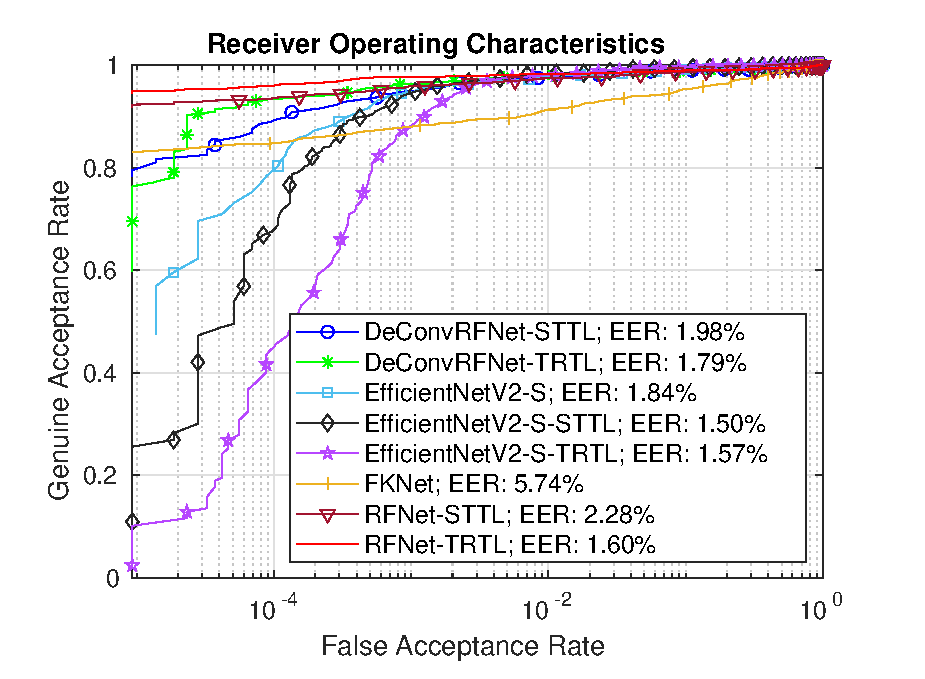
\includegraphics[width=\linewidth]{Figures/2dof3d-roc_compare_new.eps}
		\caption{}
	\end{subfigure}
	\begin{subfigure}[b]{0.45\linewidth}
		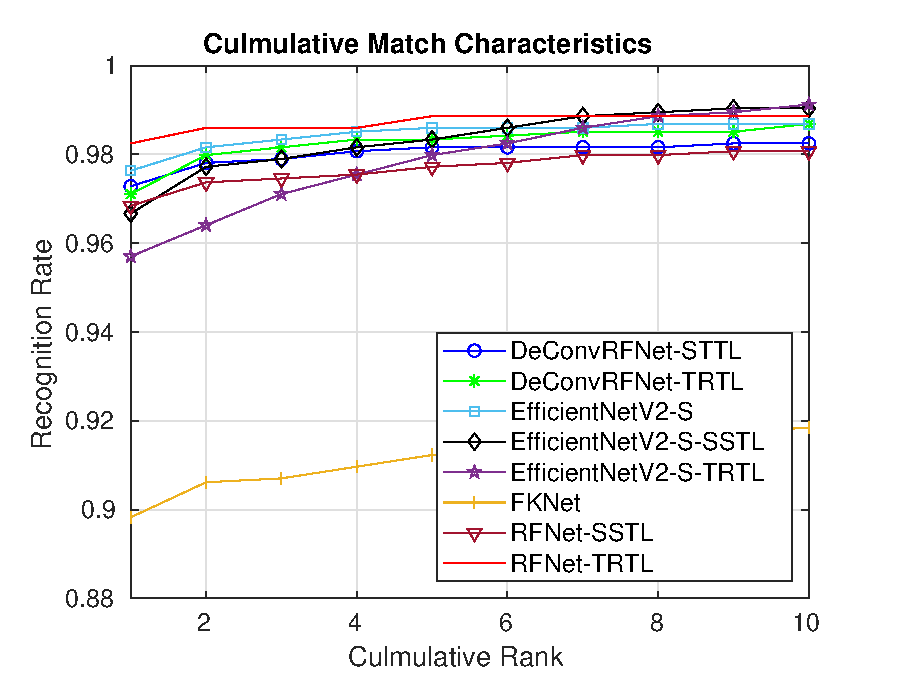
\includegraphics[width=\linewidth]{Figures/2dof3d-cmc_compare_new.eps}
		\caption{}
	\end{subfigure}
	\caption{Comparative ROC (a) and corresponding CMC (b) for one-session on the 3D finger knuckle database\cite{3dfingerknuckle}.}
	\label{2dof3d-one-session}
\end{figure}